\chapter[Ferramentas de apoio]{Ferramentas de apoio}

\section{NLTK}

Dado como um conjunto de bibliotecas para processamento de linguagem natural, o NTLK oferece interfaces de processamento para classificação, tokenização, “stemming”, “tagging” e análise. Apesar de ser uma biblioteca originalmente norte-americana (e por consequência focada no inglês), os principais módulos do NLTK contam com suporte para o português, como o stemming e o módulo de stop words.

O módulo de stemming tem como objetivo retirar o sufixo das palavras, de modo que se mantenha apenas o seu radical. Esse método aumenta consideravelmente a chance de palavras sinônimas se corresponderem \cite{marconltk}, melhorando assim a performance geral do analisador de frases. O módulo do stop word também é focado em melhorar a performance, visto que tais palavras raramente adicionam algum significado semântico à frase. Contudo, retirar estas pode indicar uma perda significativa de semântica. Apesar das suas capacidades, a biblioteca NLTK é considerada muito pesada e lenta em termos de performance, chegando até a ser considerada uma biblioteca apenas para pesquisa e exploração.

\begin{figure}[!htb]
    \center{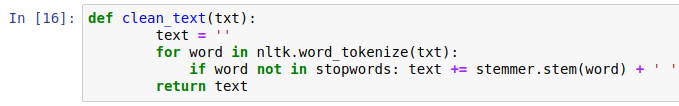
\includegraphics[scale=0.6]
    {figuras/nltk_example2.png}}
    \caption{\label{fig:my-label} NLTK aplicando técnicas de stemming e remoção de stop words}
\end{figure}

\section{scikit-learn}

A biblioteca scikit-learn provê algoritmos de aprendizado supervisionado e não-supervisionado através de interfaces pré-definidas. A SKLearn implementa todos os algoritmos de classificação considerados neste trabalho.

Além da classificação, o scikit-learn contém outros módulos, como os de regressão e clusterização. Por se tratar de uma biblioteca para mineração e análise de dados, uma série de pacotes é necessária para o seu funcionamento, como o matplotlib, o numpy e o pandas. Esses pacotes fazem parte de uma “stack” chamada Pydata. Neste projeto, todos os classificadores utilizados e testados foram providos pelo scikit-learn.

A biblioteca do scikit-learn também possui suporte para a aplicação de técnicas de treinamento e organização do código, como:

\begin{itemize}
    \item \textbf{Pipeline}: uma classe que permite a construção de métodos, compostos por diversos passos e parâmetros variáveis. Nos experimentos realizados neste trabalho, esses passos são as classes responsáveis por extrair os atributos do texto e pelo modelo da classificação.
    \item \textbf{K-fold cross-validation}: uma técnica que visa eliminar o viés gerado ao realizar a divisão do dataset entre dado de treino e dado de teste. Ela busca solucionar este problema dividindo o dataset em K partes e realizando o experimento proposto K vezes, revezando, em cada iteração, a parte a ser utilizada no teste. Observe a Figura X abaixo.
    
    \begin{figure}[!htb]
        \center{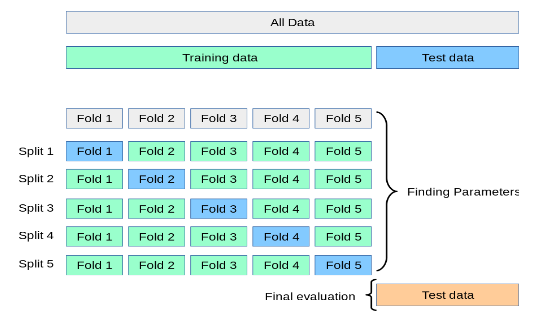
\includegraphics[scale=0.6]
        {figuras/kfold_example.png}}
        \caption{\label{fig:my-label} Demonstração visual do K-fold}
    \end{figure}
    
   \item \textbf{GridSearchCV}: uma técnica que realiza uma busca de “força bruta”, para encontrar os hiperparâmetros do modelo de classificação que melhor atendem o problema. Para isso, utilizando o scikit-learn, é definido um conjunto de parâmetros a serem avaliados e o critério de avaliação do método. O GridSearchCV, então, avalia o desempenho do modelo utilizando todas as possíveis combinações dos parâmetros sugeridos. De acordo com a documentação do scikit-learn, a busca pelos parâmetros é otimizada pelo uso da validação cruzada \cite{scikit-learn}.
\end{itemize}

\section{Jupyter notebook}

O Jupyter notebook é uma ferramenta que permite não só a execução de código python no navegador, mas também seu gerenciamento, organização e apresentação. Com ela, o desenvolvimento dos algoritmos é facilitado, visto que a execução dos mesmos pode ser separada por “blocos”. Seguindo essa mesma lógica, é possível utilizar-se de comentários e \textit{markdown} para documentar esses blocos de algoritmo, de modo que se facilite tanto a organização, quanto a leitura posterior desses dados. Com todas essas vantagens, o jupyter notebook se tornou nossa principal ferramenta para a realização dos testes. Esta também é uma ferramenta do conjunto Pydata.

\begin{figure}[!htb]
    \center{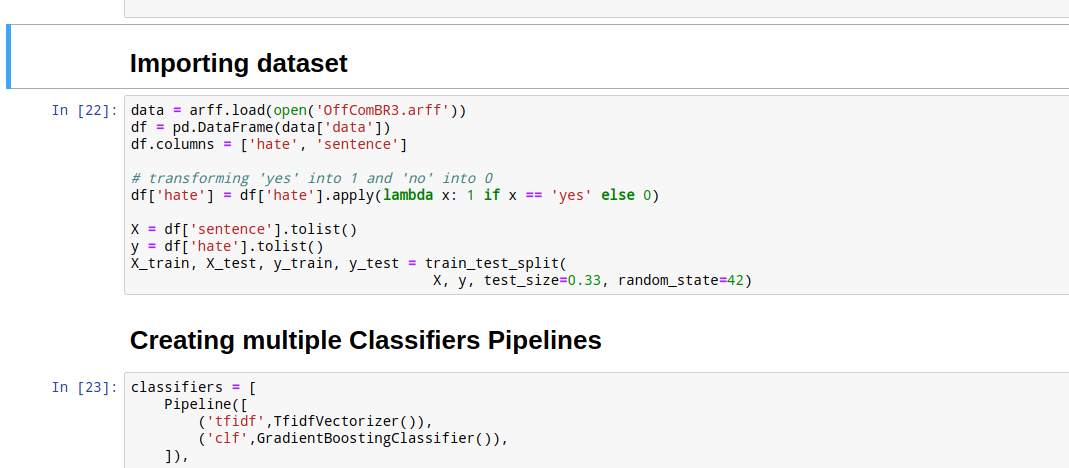
\includegraphics[scale=0.6]
    {figuras/jupyter-note.png}}
    \caption{\label{fig:jupyter} Screenshot de Jupyter Notebook}
\end{figure}

\section{Conjunto de dados}

Um dos desafios enfrentados no atual trabalho foi a busca por um conjunto de dados (dataset) categorizados de discurso de ódio que atenda aos requisitos de: ser em português brasileiro, utilizar linguagem coloquial e ser composta por textos pequenos. Estes requisitos foram definidos para que os dados utilizados nos treinos sejam o mais próximo possível dos dados onde ele pode ser aplicado.

O conjunto de dados encontrado que atende aos requisitos do projeto é o OffComBR \cite{Pelle2017}, composto por mais de mil e duzentos comentários, com cerca de 419 considerado discurso de ódio. O dataset em questão aborda diversos assuntos polêmicos, como política, economia, futebol e religião. As frases contém uma média de 72 caracteres, além de um alto grau de coloquialismo e erros de digitação. Racismo, sexismo, homofobia, xenofobia e intolerância religiosa estão entre os critérios adotados na classificação manual realizada pelos seus colaboradores.

\begin{table}[htbp]
\centering
\begin{tabular}{cccccccccc}
\hline
 & \textbf{\begin{tabular}[c]{@{}c@{}}D. ódio\end{tabular}} & \textbf{\begin{tabular}[c]{@{}c@{}}Frase\end{tabular}} &  \\
 \hline
\textit{\textbf{0}} & 1 & Votaram no PEZAO agora tomem no CZAO  \\
\textit{\textbf{1}} & 0 & So conversa mole desde que golpeou o poder nao e Temer  \\
\textit{\textbf{2}} & 0 & FORA TEMER  ABAIXO A REDEGLOBODECORRUPCAO. \\
\textit{\textbf{3}} & 1 & VAO BATE PANELASSEUS BURROSBEM FEITO \\
\textit{\textbf{4}} & 0 & Podiam retirar dos lucros dos bancos
\end{tabular}
\caption{Trechos do dataset escolhido}
\label{ngrams}
\end{table}

\begin{center}
\begin{table}[h!]
\centering
\begin{tabular}{ |c|c|c| } 
 \hline
 Tamanho & 1250 frases \\ 
 Discurso de ódio & 419 frases  \\ 
 Média de caracteres. & 72.5  \\
 Média de palavras & 12.8 \\
 \hline
\end{tabular}
\caption{Informações do dataset}
\end{table}
\end{center}


\begin{figure}[!htb]
    \center{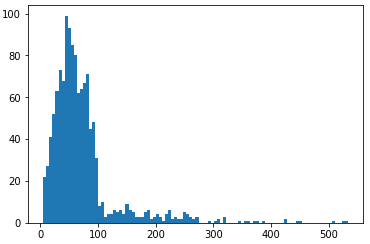
\includegraphics[scale=1]
    {figuras/dataset_info_graphic.png}}
    \caption{\label{fig:jupyter} Histograma representando a frequência de caracteres do dataset}
\end{figure}